\subsection{Angular-Acceptance Simulation For H2 Parameters}
\label{sec:angular_acceptance_simulation_for_h2_parameters}

The so-called H2 hole-ice parameters assume a hole-ice radius of
\(30\cm\), corresponding to the entire drill hole being filled with hole
ice, and a geometric hole-ice scattering length of \(50\cm\),
corresponding to an effective scattering length of \(8.33\m\).
\cite{holeicestudieswithyag}

Using the new medium-propagation algorithm (section
\ref{sec:algorithm_b}) with direct detection and plane waves as photon
sources (section \ref{sec:angular_acceptance_scan}) to generate an
effective angular-acceptance curve for these H2 hole-ice parameters:

\hspace{1cm}

\begin{center}
  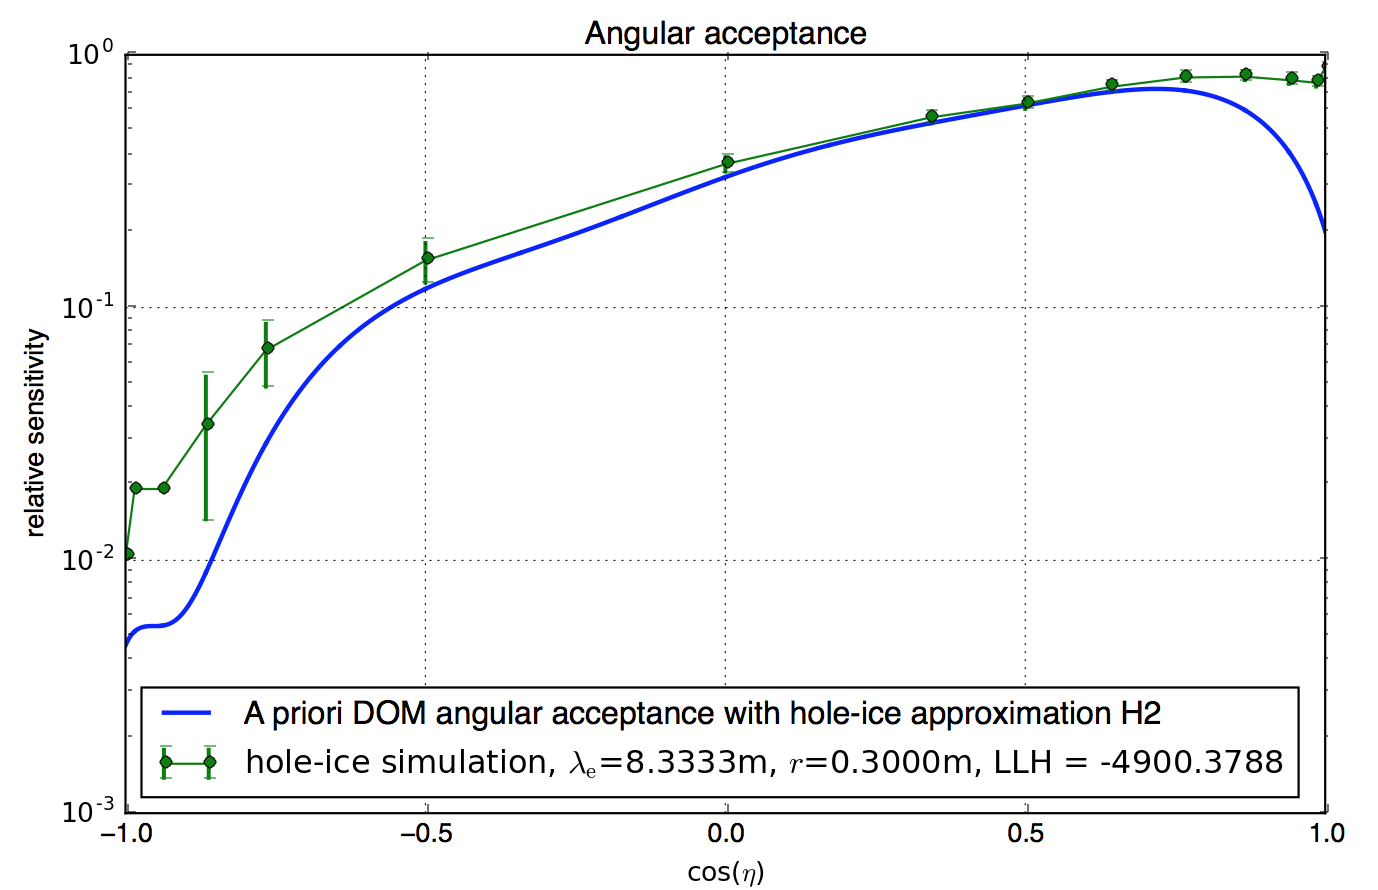
\includegraphics[width=0.75\textwidth]{img/angular-acceptance-karle-h2-vs-reference}
\end{center}

\hspace{1cm}

The blue a priori curve is based on previous \photonics simulations
assuming the same H2 hole-ice parameters. \cite{lundberg, icepaper}

\newpage

The same simulation assuming an effective hole-ice scattering length of
\(50\cm\), corresponding to a geometric scattering length of \(3\cm\):

\hspace{1cm}

\begin{center}
  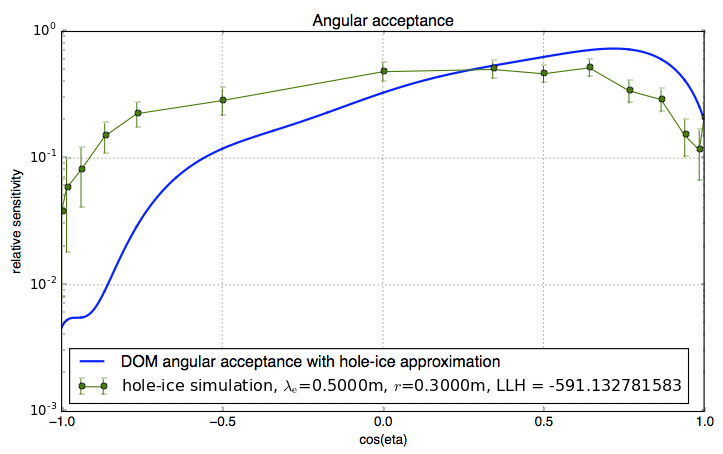
\includegraphics[width=0.75\textwidth]{img/angular-acceptance-karle-h2-assuming-esca}
\end{center}

\hspace{1cm}

\docpar{These simulations are documented in \issue{80}.}
